\documentclass[conference]{IEEEtran}

\usepackage{listings}
\usepackage[framed,numbered,autolinebreaks,useliterate]{mcode}

\lstset{language=Matlab}
%\documentclass[draftcls, 12pt,onecolumn,oneside]{IEEEtran}
\usepackage{cite,graphicx,amssymb,amsmath,color,textcomp}
\newtheorem{theorem}{\underline{Theorem}}%[section]
\newtheorem{lemma}{\underline{Lemma}}%[section]
\newtheorem{remark}{\underline{Remark}}%[section]
\ifCLASSOPTIONcompsoc
  % IEEE Computer Society needs nocompress option
  % requires cite.sty v4.0 or later (November 2003)
\usepackage[nocompress]{cite}
\else
\usepackage{cite}
\fi
\newcounter{mytempeqncnt}

\begin{document}


\title{The Distribution of the Sum of Independent and Identically Distributed Random Variables}
\author{Zilong Wang 18281218\\wangzilong@bjtu.edu.cn

 }


\maketitle
\begin{abstract}
In this paper, the problem of the sum of independent and identically distributed random variables are studied, which should obey normal distribution by using Central Limit Theorem. Simulations are provided to corroborate the proposed studies.
\end{abstract}

% Note that keywords are not normally used for peerreview papers.
\begin{IEEEkeywords}

\end{IEEEkeywords}



\section{Problem description}
\subsection{Central Limit Theorem\cite{b1}}
In probability theory, the central limit theorem establishes that, in some situations, when independent random variables are added, their properly normalized sum tends toward a normal distribution even if the original variables themselves are not normally distributed. The theorem is a key concept in probability theory because it implies that probabilistic and statistical methods that works for normal distributions can be applicable to many problems involving other types of distribution.

Mathematically, if $X_1, X_2, ..., X_n$ is a random sample of size $n$ taken from a population with mean $\mu$ and finite variance $\sigma^2$ and if $\bar{X}$ is the sample mean, the limiting form of the distribution of $Z=\frac{\bar{X}_n-\mu}{\frac{\sigma}{\sqrt{n}}}$ as $n\to \infty$, is the standard normal distribution.

\subsection{Our Work}
We produce $100$ sets of independent and identically uniform variables $x_1, x_2, ..., x_{100}$ from a population of uniform distribution variables whose range is between $(-2,2)$. Then we calculate $\sum_{i=1}^{100}x_i$ as $s$. We do this procedure for $10^4$ times and we write a MATLAB code to simulate it.Then we test and find that $s$ obeys normal distribution by using Central Limit Theorem. 



\section{Simulation Process and Results}
We produce $x_1, x_2, ...,x_{100}$ and adding them up then do it for $10^4$ times, and drawing its histogram.
\begin{figure}[htbp]
\centering
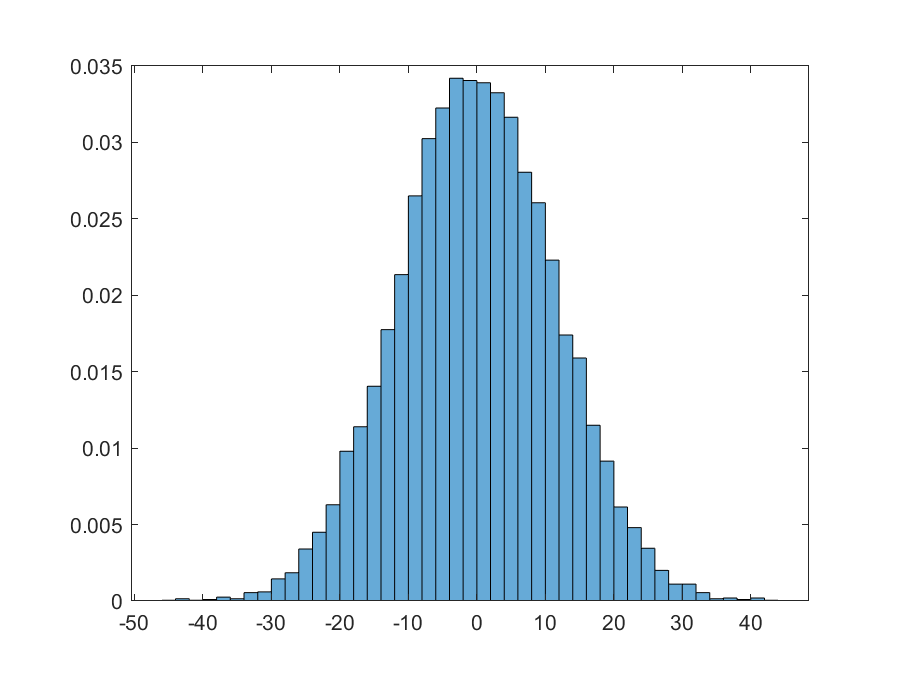
\includegraphics[height=48mm,width=64mm]{Histogram.eps}
\caption{Histogram of $s$}
\centering
\label{fig:System_Model} \vspace{2mm}
\end{figure}

Cause $x_{i}$ obeys uniform distribution, where $\mu = 0, \sigma = \frac{4}{3}$ when $s = \sum_{i = 1}^{100}x_i$. By using central limit theorem, we know that the sum of $s$ obeys $N$~$(0,\frac{160000}{9})$. Meanwhile, we can plot the probability density function of $N$~$(0,\frac{160000}{9})$.

The density function of normal distribution is

\begin{align}
	f(x)=\frac{1}{\sqrt{2\pi}\sigma}exp\left(-\frac{(x-\mu)^2}{2\sigma^2}\right)
\end{align}

In this problem, the density function of normal distribution is
\begin{align}
	f(x)=\frac{\sqrt{3}}{20\sqrt{2\pi}}exp\left(-\frac{3 x^2}{800}\right)
\end{align}



\section{Findings}
Comparing the distribution of $s$ and a standard normal distribution, we find the distribution of $s$ may obey normal distribution. Then by the calculation of Central Limit Theorem, we verify the sum of independent and identical variables obey distribution.

\begin{figure}[htbp]
\centering
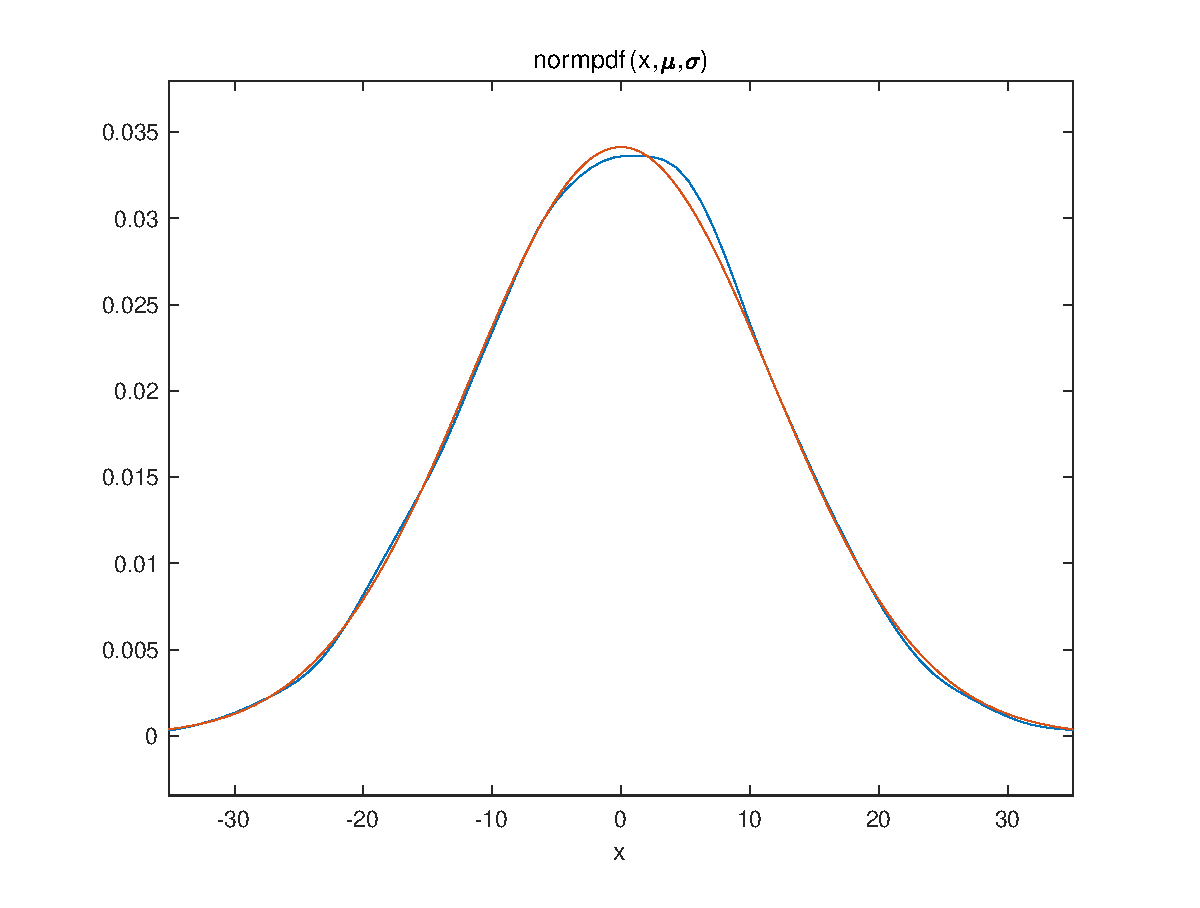
\includegraphics[height=48mm,width=64mm]{distribution.eps}
\caption{Normal Distribution and simulated distribution. }
\centering
\label{fig:System_Model} \vspace{2mm}
\end{figure}

\bibliographystyle{IEEEtran}
\begin{thebibliography}{00}
\bibitem{b1} Montgomery, Douglas C.; Runger, George C. (2014). “Applied Statistics and Probability for Engineers (6th ed.)”. Wiley. p. 241. ISBN 9781118539712.
\end{thebibliography}





\end{document}



